\documentclass[12pt]{article}

\usepackage{amsmath,amsfonts,amssymb}
\usepackage{graphicx}

\newcommand{\gcc}{\texttt{gcc}}
\newcommand{\foptinfo}{\texttt{-fopt-info-<val>-vec}~}
\newcommand{\Othr}{\texttt{-O3}~}
\newcommand{\restrict}{\texttt{restrict}~}
\newcommand{\const}{\texttt{const}~}
\newcommand{\double}{\texttt{double}~}

\newcommand{\A}{\texttt{A}~}
\newcommand{\B}{\texttt{B}~}
\newcommand{\C}{\texttt{C}~}

\title{CS 267 Assignment 1 Report}
\author{Maxim Rabinovich and Josh Tobin \\ Team 30}

\begin{document}

\maketitle

\section{Overview}

We implemented most of the suggested optimizations and found that copy optimization and explicit vectorization produced the most significant performance gains. We found that our optimizations (other than parameter tuning) produced a similar performance improvement when run on a Macbook Air with a 1.4GHz core i5 processor.

\section{Optimization strategies and rationales}

We describe our optimizations roughly in the order in which we attempted them. We initially thought {\bf loop reordering} and {\bf loop unrolling} might lead to
improved performance by themselves because they would lead to improved locality in memory accesses and a greater chance of auto-vectorization and other compiler optimization. Unfortunately, we found that loop unrolling provided no measurable benefit and loop unrolling gave a bump of only about $2\%$ (absolute),
bringing our number up to about $10\%$.

After adding the \foptinfo flag to \gcc, we realized that the compiler was not performing any {\bf autovectorization}. We therefore added the \Othr flag and, after
some online research, the \texttt{-funsafe-math-optimizations}, \texttt{-msse},\texttt{-msse2}, and \texttt{-mavx2} flags. We also gave \C the \restrict attribute and flagged all other variables
as \const (making \A and \B \const pointers to \const). With these changes in place, \gcc~successfully vectorized the inner loop of the block matrix multiplication step and our performance jumped to about $15\%$.

We then revisited the {\bf loop reordering} strategy, reasoning that ensuring that accesses to the \A and \B in the innermost preserved locality (in particular, by
accessing contiguous elements successively) would lead to improved cache utilization and therefore to improved performance. We did in fact observe a significant performance bump from this strategy, moving up to about $20\%$ of peak performance.

At this point, a glaring remaining issue was that, although the blocks were small enough to fit into cache, it might nonetheless not be possible to store them in the
cache simultaneously because of their discontiguity in memory---a degree of discontiguity determined by the size of the matrix, not by the block size or other parameters under our control. We therefore implemented a {\bf copy optimization} procedure that copied \A and \B into a new buffer in which the blocks were
ordered in column major, but each block was stored contiguously in memory (as either row major or column major, with the optimal choice varying from version to version of our code---we omit these details for the sake of brevity). This gave a significant bump up to $25\%$.

By far the greatest gains came from switching to {\bf compiler intrinsics}. We tried both {\bf SSE} and {\bf AVX} and obtained good results from the first and
outstanding results from the second. Inspired by the matrix multiplication example in the hints, we reasoned that explicit vectorization with SSE could be used to drastically speed up the multiplication of 
$2 \times K$ and $K \times 2$ pieces of \A and \B, where $K$ is as in the provided code (i.e. the block size, except in corner cases) by ensuring that two multiplications happened in one instruction and 
likewise with add operations and read and write operations on \C. The performance gain from SSE ended up being notable, namely $5\%$, bringing us up to $30\%$. Applying the exact same strategy but with AVX,
we reached $46\%$ performance immediately.

We note that in order to use compiler intrinsics, we needed to ensure that our matrices were aligned on 16-byte (SSE) or 32-byte (AVX) boundaries. We achieved this by allocating aligned memory during our copy optimization procedure and initially experimenting
only with matrix sizes that were powers of two.\footnote{To enforce alignment, we added \gcc's intrinsic \texttt{aligned} attribute to \A and \B.} 
This necessitated an eventual generalization to the case where the matrix sizes were arbitrary, which we dealt with by always assuming the block size is a multiple of $4$ (which, since a \double has size 8 bytes, ensures
that all the relevant entries are properly aligned for AVX access. We omit the details because they are complicated to explain in words. Part of this process required rounding the matrix size up to the nearest multiple of the block size, which led to some issues we discuss more below.
It also created some corner cases, since we could not write into \C out of bounds.\footnote{Actually, technically we could because more memory was allocated by the benchmarking script than was needed, but we made sure to avoid doing so.} When $4$ rows/columns were no longer available,
we backed off from AVX to SIMD and, when $2$ were no longer available, to the base loop reordered block multiply from above. We suspect optimizing the corner cases could've led to an even further gain in performance, but we did not investigate this issue deeply. All in all, the end point of this process
were results around $46-47\%$.

Finally, we implemented a second level of copy optimization to attempt to optimize L2 cache performance. We did this by storing the matrices in column major over outer blocks, then storing each outer block contiguously, in row/column major (as needed) over the inner blocks, with each one stored contiguously as before.
This led to a performance bump up to $48.6\%$, our final number.

Throughout most of the assignment, we kept the inner block size at $32$. This is a reasonable choice, since Edison's L1 cache has 32 KB of storage for data, which corresponds to an optimal block size (based on $3B^{2} = 4000$) of $B \approx 36$. We tried bumping up the block size to $36$ but observed a slight dip in
performance, so we reverted to the old value. The outer block size was $64$. This is again a reasonable choice, although probably not optimal, since Edison's L2 cache has 256 KB of storage, meaning that the optimal $B$ would be around $2\sqrt{2} \cdot 36 \approx 102$. We didn't find any benefits from making the outer
block larger, however, after a few brief experiments, so we again reverted to the old value.

\section{Evaluation on other machines}

We tested our code on a Macbook Air with a 1.4GHz core i5 processor. Without adjusting the code or parameters chosen, our implementation increased performance from about 6.5\% for the naive blocked implementation to about 40\%,  
which is comparable to the performance gain seen on Edison.

\section{Discussion of performance dips}

% Add plot of results versus size.
\begin{center}
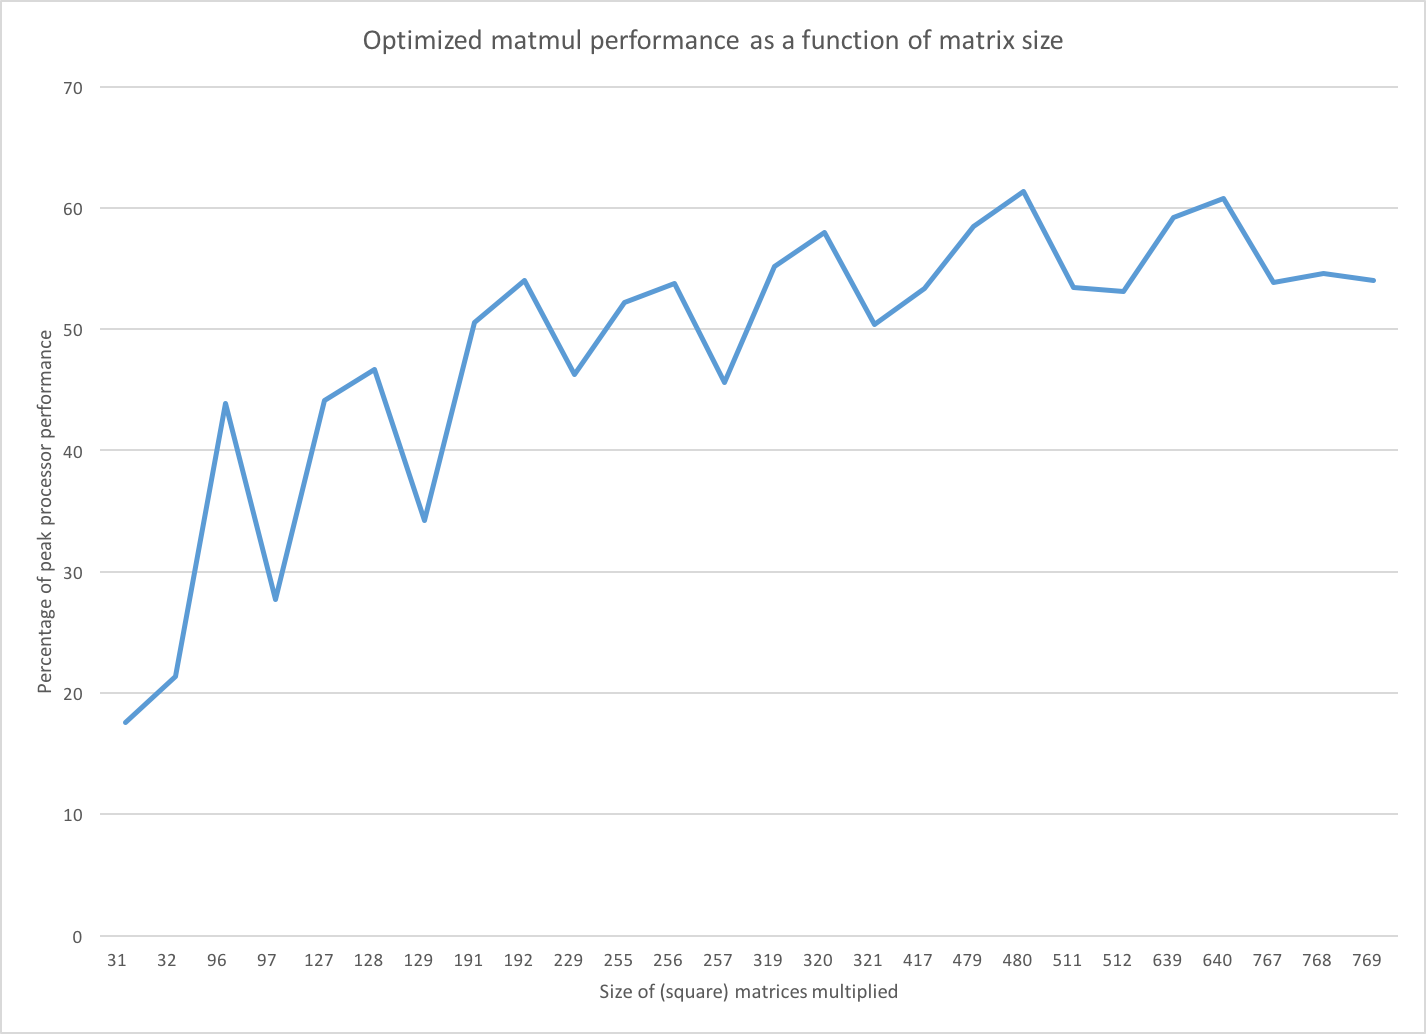
\includegraphics[scale=0.5]{chart}
\end{center}

Unsurprisingly, given our utilization of copy optimization and our rounding up of the matrix sizes, our code performed best on the larger instances, specifically those of size at least $192$ (or thereabouts). Performance dipped in particular on values that were just above multiples of the block size, since in this case
our rounding adds a comparatively large amount to the matrix, leading to overhead both for initial copying---which, however, we would expect to be negligible at that scale, but we aren't entirely sure---and in the number of loops executed by the program. An alternate explanation for the dip is that adding just one to
a multiple of the block size creates problems because it is guaranteed to trigger a call to a block multiply involving a $1 \times K$ matrix, which is done using the slowest backoff method.

\end{document}